\section{Architecture for Embedded Software Verification}
\label{architecture_s}	
Figure~\ref{architecture} presents the proposed overall architecture for ensuring Java bytecode correctness. 
\begin{figure}[ht!]
\begin{center}
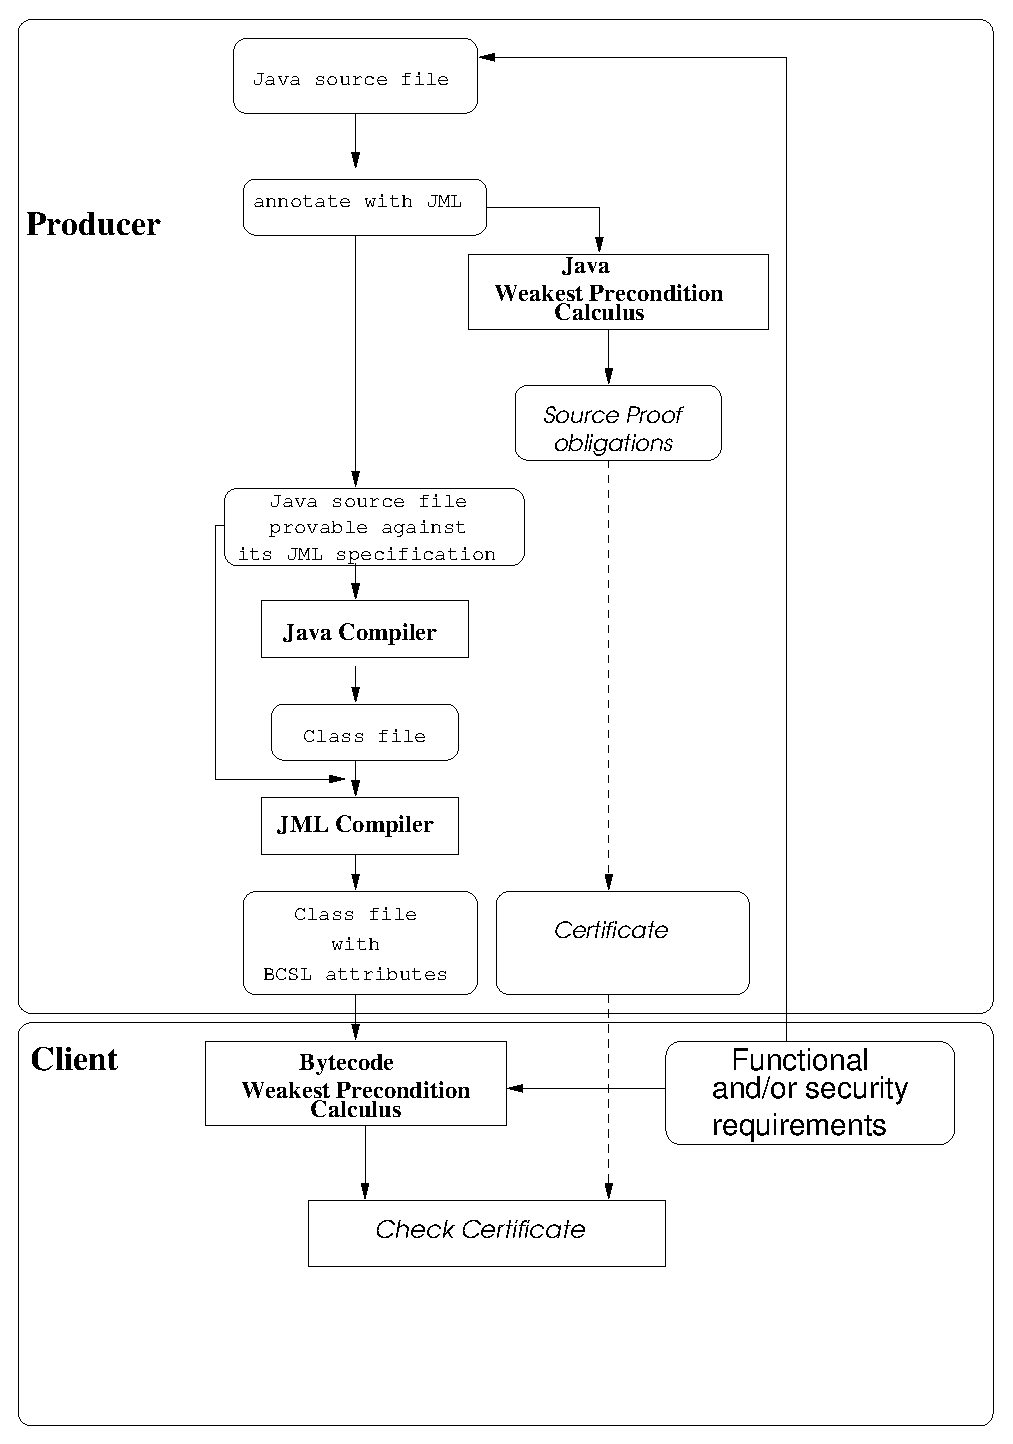
\epsfig{file=architecture.eps, width=\linewidth}
\caption{The overall architecture for annotating and verifying code}
\todo{change in the figure the box that says class with JML attributes}
\label{architecture}
\end{center}
\end{figure}
It describes a process that allows a client to trust a code produced by an untrusted code producer.

%\todo{Lilian, c'est ce que tu veux dire ? }
In the first stage of the process the client provides the functional and (or) security requirements to the producer. The requirements can be in different form:
\begin{itemize}
\item A specified interface that describes the application to be developed. In that case, the client has fully specified in JML the features that have to be implemented by the code producer.
\item An API with some restricted access to some method. In these case, the client can protect its system by restricting its usage (for example: ...). 
\end{itemize}
The producer uses Jack to check the requirements and usually has to add JML annotations for this %In both cases, the code producer develops its application and proves that it fulfills the given requirements using Jack; %in most cases, to complete this task, some annotations have to be added to the code 
e.g. loop invariants, assertions at particular program points. Only then have we got the annotated Java source files to feed to the JML compiler.
%Thus the burden of annotating the code 
%in order to render it provable w.r.t. the client requirements is left to the producer. 

When the annotations are sufficient to prove the code, 
the Java file is then normally compiled with a Java compiler to obtain a 
class file. 
This class file is then annotated with special JML attributes extracted from the source file. 
At this stage, the Java class files contain all the information that will allow the client to check it (e.g. loop invariants). 
 
In particular 
the client will generate proof obligations from the untrusted annotated bytecode and his security requirements 
(expressed in a suitable form)
 as shown at fig. \ref{architecture}. Proof obligations are formulas which, if provable, guarantee the bytecode correctness.
The latter are then proved, for instance, with the JACK framework. If the client succeeds in proving 
the verification conditions, he can trust the unknown code. 

In this framework, it is not necessary for the client to have an access to the source to verify high level properties. 
Nevertheless those properties can be expressed easily at source level.

To implement this framework, we have defined an extension of the class file format, we have implemented a tool to insert 
those special attributes in the class file and we have extended the Jack framework to generate proof obligations at bytecode 
level and to prove them with the plugged Jack provers (as explained in the introduction). 
The coming sections introduce those features.  

